\documentclass[11pt,letterpaper]{article}
\pagestyle{plain}
\usepackage{alltt}
\usepackage{amsmath}
\usepackage{amssymb}
\usepackage[utf8]{inputenc}
\usepackage{times}
\usepackage{hyperref}
\usepackage{graphicx}
\usepackage{wrapfig}
\usepackage{listings}
\usepackage[usenames,dvipsnames]{xcolor}
\usepackage{setspace}
\usepackage{python_syntax}
\usepackage{natbib}
\usepackage{bibentry}
\usepackage{todonotes}
\usepackage{url}
\usepackage[compact]{titlesec}
\usepackage{enumitem}
\usepackage[
top    = 1in,
bottom = 1in,
left   = 1in,
right  = 1in]{geometry}
\linespread{0.92} % NSF allows up to 6 lines per inch.  
\def\UrlFont{\em} % Italicize all URLs.  
\frenchspacing
\setlist{nolistsep} % or \setlist{noitemsep} to leave space around whole list
\lstset{ %
	basicstyle=\footnotesize\ttfamily,
	breaklines=true,
	language=Python,
	}
\let\verbx\lstinline
\newcommand{\bfhead}[1]{\noindent \textbf{#1:}}

% Josh: A lot of the *potential* and actual features of SciDash are
%scattered throughout the document. This gives the reader the feeling
%that its features aren't fully thought out. 

\begin{document}

% Section 1.
\section{Introduction}

\lstinline{This is a test.}
Scientists construct quantitative models to explain observations about natural systems in a coherent and rigorous manner. These models can be characterized by their scope and validity. The scope of a model is the set of observable quantities that the model can generate predictions about, and the validity of a model is the extent to which these predictions agree with empirical observations of those quantities. Today, as the number of models and the quantity of empirical data increases, scientists face a grand challenge: efficiently discovering models whose scope is of interest and characterizing their validity against a continually growing body of available evidence. 

A new model is typically proposed by publishing a description of how it works along with an argument justifying its utility to some targeted scientific community. This argument is made in words, supported by a handful of relevant equations and figures, and judged by peer review. Ideally, reviewers ensure that the model's predictions are consistent with the available and relevant data and compare each model against previously published models. This job is becoming increasingly difficult; although authors may refer to relevant experimental data and provide citations into the literature, these are generally incomplete and biased, in that authors often focus on data favorable to their models and compare them to implausibly simple hypotheses.

If modeling papers contained detailed comparisons to all related experiments and competing models, publications would become encyclopedic and their main points obscured. A strength of model publication today is its focused description of how a model works and its conceptual and technical advances. A weakness, however, is that evaluating the scope and validity of a model is intractable using a publication alone. Publications tell us \textbf{how} a model works but are less effective at comprehensively reporting \textbf{which} goals it achieves and \textbf{how well} it achieves them. This problem is exacerbated as more data is gathered following publication. Although model validity may change in light of this new data, there is no systematic process in biology \todo{Here we mention biology, but before said "science".  Should the transition be more graceful?}today for re-evaluating existing models. Although new data and its most important theoretical implications propagate informally through a scientific community or appear in periodic reviews, the original publications -- a resource of first resort for new scientists and onlookers -- are cited "as-is'' in perpetuity. 	

We can distill the central problem discussed here as this: the process of scientific model validation today is not sufficiently rigorous, comprehensive, or ongoing. This hampers scientists' ability to make accurate predictions about experiments, compare models, and precisely identify outstanding research problems. To overcome these obstacles, we propose systematizing the model validation process by creating software and associated cyberinfrastructure dedicated to scientific model validation, supplementing today's system of peer-reviewed scientific publications to better support the modern shift toward science at a large scale.

\subsection{Existing Efforts}\label{sec:existing_efforts}
There are several well-developed facilities for data and model sharing in biology, but few if any facilitate evaluation of models against data directly.  For example, the Collaborative Research In Computational Neuroscience (CRCNS) data-sharing website \cite{crcns_url}, and the Open Source Brain (OSB) repository \cite{osb_url} are facilities for data and model sharing in neuroscience, respectively.  The CRCNS website hosts several excellent data sets of relevance to computational models; however, the data is not organized or annotated to indicate which models may be capable of predicting that data, nor how well they do.  The OSB is a resource for standardized model descriptions that permit reliable execution. Models are published as-is, without any information about which specific data the published models aim to predict and how well they achieve their goals. We aim to bridge resources like these, increasing the usefulness of each in turn.

There are related efforts in the machine learning community to develop models and validate them against standardized, publicly-available datasets according to well-specified metrics. Kaggle \cite{kaggle_url} drives model development by organizing competitions where training data is made public and competitors submit competing algorithms, compared automatically by cross-validated accuracy on an unrevealed test set. The success of Kaggle \cite{carpenter_may_2011} shows that open competitions are effective, and that this paradigm of ``modeling as a competition'' attracts data scientists across traditional discipline boundaries. However, models developed in this way fit only a few general cases in machine learning: classification, regression, and clustering. The validation criteria are straightforward in these domains. Discipline-specific competitions having a similar structure but with more sophisticated validation criteria within biology have also resulted in important advances. For example, the quantitative single neuron modeling competition \cite{jolivet_quantitative_2008} has helped us understand the complexity-accuracy tradeoff among reduced models of excitable membranes; the "Hopfield'' challenge \cite{hopfield_what_2000} famously illustrated the challenges of identification\todo{this doesn't mean anything to me, clarify?} facing computational neuroscience; the Diadem challenge is advancing the art of neurite reconstruction \cite{diadem_url}; and examples from other subfields of biology abound \cite{dream_url}. Our challenge is to develop a general framework in support of distributed, data-driven model validation workflows, in the flavor of these kinds of competitions, but where the validation criteria themselves are also specified collaboratively. Initially, we will focus on validation challenges in the biological sciences, particularly neuroscience. 

% Section 2.
\section{Outcomes and Products}
Our framework is organized around simple executable \emph{validation tests} that compute agreement between a prediction generated by a computational model and an experimental observation. The scope of a model is identified with the set of tests that a model is capable of taking and validity is identified with the set of these tests that the model successfully passes. This methodology is inspired by the ubiquitous practice of \emph{unit testing} in software engineering. A unit test evaluates whether a portion of a computer program (often a single function) meets a simple correctness criterion. A suite of such tests \emph{covering} desired program behaviors validates overall program functionality. Due to the narrow scope of each test, failed tests help precisely identify which parts of a program are not functioning correctly. Developers often write unit tests before writing the program itself, following a methodology called test-driven development (TDD) \cite{beck2003}. By writing them early, tests serve as a partial program specification, guiding its development. This allows developers to measure progress simply by looking at the proportion of tests that pass at any point during development. When modifications are made, developers can be confident that \emph{regressions} have not appeared by ensuring that that all tests that passed before a change continue to pass after it.  \todo{Add examples of successful PL test suites?}The success of unit testing and TDD in practice suggests that validation testing may be a \emph{practical} approach to systematic model validation. 

\begin{wrapfigure}{r}{0.55\textwidth}
\vspace{-0px}
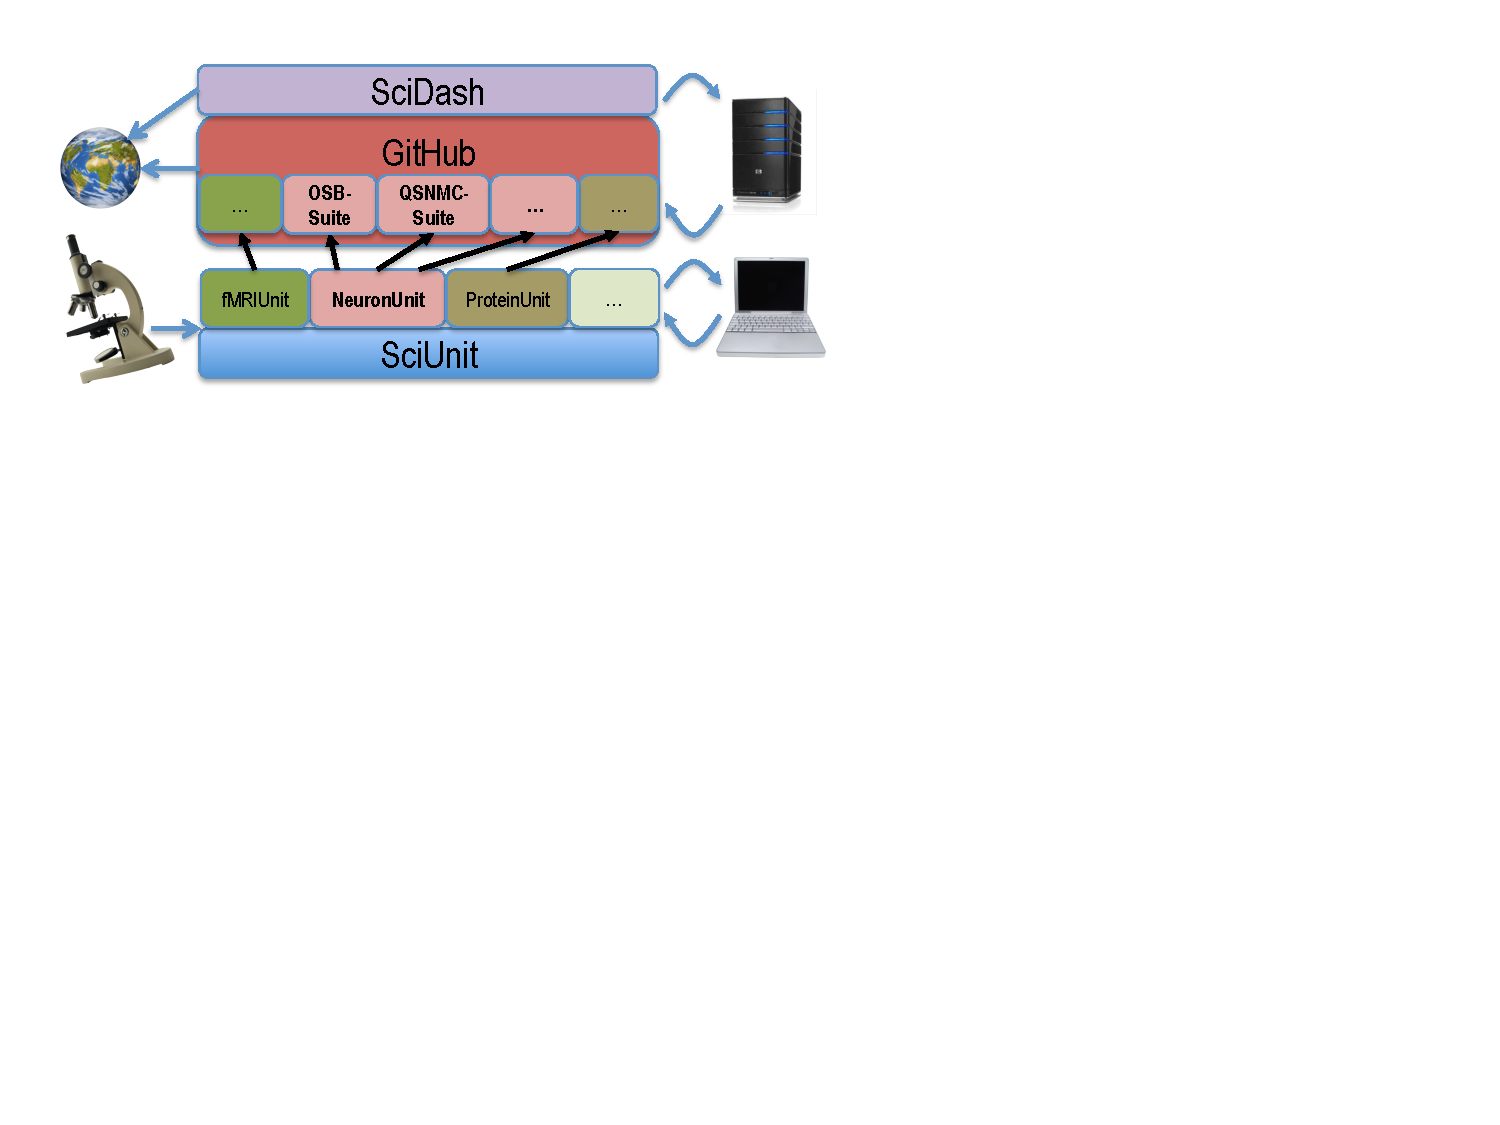
\includegraphics[scale=0.65]{sciunit_overview.pdf}
\caption{Proposal overview. \scriptsize{i) The \textit{SciUnit} framework can generate discipline-specific libraries of tests and model interfaces.  \textit{NeuroUnit} is proposed and described here.  Experimental data guides test development; model generation informs and is informed by the collections in a \textit{SciUnit} library.  Each \text{SciUnit} library on GitHub is indexed by the \textit{SciDash} web application.  \textit{SciDash} automatically runs the test collections in each library and publicly displays the results.}}
\vspace{-10px}
\label{fig:sciunit_overview}
\end{wrapfigure}
\leavevmode

\subsection{Example: Neural Membrane Potential Dynamics} To make our proposal concrete, we will begin by describing an example test related to  neuroscience. Our test is derived from experiments where a stimulus was delivered to neurons of a particular type, in the form of somatically injected current (reported in pA), while the somatic membrane potential of each stimulated cell (reported in mV) was recorded and stored.  A model that claims to have captured the dynamics of this cell type's membrane potential must be validated in several ways, but one simple test (among many) of that claim would check for correspondence between the distribution of the number of action potentials produced by the model (called a \emph{spike count}) and the distribution observed in the data, in response to the same stimuli. This test would ask any candidate model being tested to produce a predicted spike count for each stimulus and check whether the prediction fell within the empirically-observed distribution of action potential counts observed in response to that input current.  The specific metric for success would be specified by the test creator.  For example, models that, for each input current, produce action potential counts that fall with the 95\% confidence interval of the empirical data distribution might pass our example test. Importantly, this choice is made explicit in the specification of the test, so modelers need not guess which criteria potential reviewers have used to (in)validate their model.

\subsection{Validation Testing with \emph{SciUnit}} 
The first product of this proposal is a simple validation testing framework to support examples like the one above. This framework, called \emph{SciUnit}, is written in Python and is designed to make test construction (from data) and execution as easy and flexible as possible. Testing in SciUnit proceeds in three phases (Figure 1):\todo{this spacing seems unnecessarily small}
\begin{enumerate}
\item Capability Checking: The test checks to see that the model is capable of taking the test; i.e., that it exposes the needed functionality for the execution phase to proceed.
\item Test Execution: The model is executed to produce the model output by interacting with its supported capabilities.  If the model is described according to a standard specification, e.g. NeuroML, this corresponds to loading it into a supported simulator and executing it. 
\item Output Validation: The model output is compared to empirical data to determine whether the model passes.  This comparison can be of several types: for deterministic models, we may extract a matching quantile from a data distribution; for stochastic models, we may compute a measure of agreement between model output and data distributions, e.g. the Kolmogorov-Smirnov statistic.  Validation is ultimately pass/fail, but in some cases the result generated in this phase also includes a continuous statistic so that models can be ranked based on their test results in a more fine-grained manner.   
\end{enumerate}
\todo{Fix figure reference}

A validation test in SciUnit is an instance of a Python class implementing the \verbx{sciunit.Test}\todo{use a better tt font} interface. Classes that implement this interface must contain a \verbx{run_test} method that receives a model as input and produces a normalized score as output. The capabilities that the model must possess in order for the test to operate correctly are given using the \verbx{required_capabilities} attribute. In many cases, several tests will have a similar form, differing only by a choice of parameters or by association with a particular dataset. Such parameterized test families correspond to subclasses of \verbx{sciunit.Test} that take the needed parameters as constructor arguments. 

\begin{figure}
\caption{A single neuron firing rate test implemented in \textit{SciUnit}}
\label{fig:rate_test}
\begin{python}
class RateTest(sciunit.Test):
	def __init__(self, mean, std, input_current):
		self.mean, self.std, self.input_current = \
		mean, std, input_current
	
	required_capabilities = (
		neurounit.Capabilities.ReceivesCurrent,
		neurounit.Capabilities.ProducesFiringRate
	)
	
	def run_test(self, model):
		model.set_current(self.input_current) 
		# Implementation guaranteed by capability check.  
		rate = model.get_firing_rate()
		
		mean, std = self.mean, self.std
		result = (mean - std) <= rate <= (mean - std)
		return sciunit.scores.BooleanScore(result, related_data={
			"rate": rate,
			"mean": mean,
			"std": std
		})
\end{python}
\vspace{-18px}
\end{figure}

In the example from Figure \ref{fig:rate_test}, the RateTest class implements a parameterized family of tests that compare the output firing rate (action potentials per second) of a neuronal model, driven by a given somatic input current, to an empirically measured mean and standard deviation of the rate derived from a set of replicated experiments. The test produces a boolean score indicating agreement within one standard deviation of the empirical mean. The input currents, mean, and standard deviation are provided as constructor arguments on line 2 (constructors are named \verbx{__init__} in Python.) On lines 5-8, the required capabilities are listed: the model must be able to take a current as input and produce firing rates as output. These capabilities are used in the \verbx{run_test} method, on lines 11 and 12 respectively, to execute the model against the provided current. The resulting firing rate is compared to the empirical mean and standard deviation on line 15 and a boolean score is produced on lines 16-20. In addition to the boolean value itself, the score also contains metadata that may be useful to scientists wishing to examine the result in detail. In this example, we save the model's output rate and the provided mean and standard deviation alongside the result, by specifying the \verbx{related_data} parameter.  \todo{Can the test output a standard measure of agreement in addition to the boolean value and the related data?}

To create a validation test, a scientist instantiates the RateTest class with a particular mean, standard deviation and input current (I, not shown):

\verbx{mitral_cell_rate_test = RateTest(mean=18.0, std=40.0, input_current=I)}

The test is then executed against a model instance (described below), using the sciunit.run function:

\verbx{score = sciunit.run(mitral_cell_rate_test, synchrony_model)}

The sciunit.run function operates in three phases, implementing the abstractions at the beginning of section 3:
(1)	Capability Checking: The model is verified as capable of taking the test by checking each capability in the test's \verbx{required_capabilities} attribute.
(2)	Test Execution: The test's \verbx{run_test} method is called to execute the model and cache output.
(3)	Output Validation: \verbx{run_test} returns an instance of a \verbx{sciunit.Score} subclass containing a goodness-of-fit metric between the model output and the data used to instantiate the test.

Any errors that occur during this process are reported by raising an appropriate exception.

\subsection{Test Suites}
A test suite is a collection of tests designed to validate a model against several mutually coherent requirements:

\noindent
\verbx{urban_tests = sciunit.TestSuite([mitral_cell_rate_test, \}

\noindent
\verbx{                                 mitral_cell_interval_test])}

When a test suite is executed against a model, it produces summary data that can be shown on the console or visualized by other tools, such as the web application described in the next section.

\subsection{Community Workflow}\todo{Maybe this section should be moved to the end of the introduction}
Unit tests are produced by the community of developers involved in the development of a program. Correspondingly, members of a scientific community can collaboratively produce suites of validation tests in common source code repositories. Each test specifies the model requirements, and provides a procedure for determining whether a candidate model (the input to the test) is consistent with a particular summary of experimental observations (the parameters of the test). Model performance on a collaboratively curated suite of validation tests can serve as justification of claims regarding the model's validity as a description of the scientific system characterized by the test suite.
This workflow continuously produces a summary of the field indicating which models are capable of taking each test, i.e. whether the test falls within the model's scope, and for each capable model, how well it performed, i.e. its validity.  Model usefulness becomes a function of the weight given to each test, determined per investigator or by community consensus. This test-driven scientific workflow leverages the desire of modelers to promote their models' virtues -- test suites represent clear \emph{challenges}, issued by experimentalists to the community, and passed tests certify success for the modelers. As more data is gathered and test suites are refined, past models can be tested continuously againt current empirical knowledge, in a fully-automated manner because the interface between tests and models is fixed.  

\subsection{\textit{SciUnit}: A Simple Validation Testing Framework}\todo{Maybe this section should be the start of "Outcomes and Products"}
Conceptual and practical simplicity -- the absence of "heavy-lifting'' -- is an essential requirement for community participation. Our design does not require the release of raw data or storage in standard formats. Instead, salient aspects of the data are abstracted away behind a test definition. Similarly, implementation details of a model (e.g. its programming language) need not be public or standardized -- the implementation must simply be wrapped to expose a standardized interface, so that tests can access model capabilities. Each community can collaboratively specify model interfaces capturing high-level operations of their preferred modeling formalisms. Existing modeling standards (e.g. NeuroML \cite{neuroml_url,gleeson_neuroml:_2010}) and interface definition languages (IDLs) \cite{bachmann2008}\todo{Fix reference} are leveraged to simplify this process. \textbf{Thus, the first product of this proposal is an object-oriented validation testing framework called \textit{SciUnit}, written in Python, that makes test construction (from data) and test-driven model execution easy and flexible.} 

\subsection{\textit{SciDash}: A Community web application}\label{sec:scidash}
This framework is most effective when the current state of a research area is represented by a collection of tests and models. This requires coordination among research groups, so community-oriented cyberinfrastructure to support test suite creation and summarization, building upon \textit{SciUnit}, is essentiall. We propose a service, called \textit{SciDash}, utilizing existing infrastructure for coordinated development of software repositories, focusing on GitHub \cite{github_url} \cite{ram_git_2013}. A suite of related tests will be contained in a GitHub repository with a stereotyped high-level structure that allows the \textit{SciDash} web application to discover, index and summarize it on an ongoing basis (Fig. \ref{fig:scidash_repo}). The portal, a web application written using the pythonic Django framework \cite{django_url} will serve as a central location where scientists can discover relevant test suites, determine test requirements, and summarize the results of test execution on submitted models. Test results can be visualized as a "record matrix" composed of large numbers of model/test combinations (Table \ref{table:record_matrix} provides a toy example).  Each row in this matrix will contain results for all tests taken by one model and would serve as clear evidence of that model's scope and validity.  Models, tests, and records will be stored on GitHub, pointed to by hyperlinks in the record matrix. \textit{SciDash} will serve as a public record of competition among models, facilitating and encouraging data-driven development among modelers. \textbf{Thus, the second product of this proposal is a web application called \textit{SciDash}, whose back-end can index test suite repositories collaboratively developed on GitHub, and whose front-end offers users a simple environment for discovery and evaluation of models, tests, and results.}  

\begin{wrapfigure}[18]{r}{0.5\textwidth}
%\centering
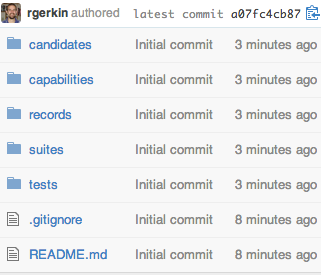
\includegraphics[scale=0.7]{scidash_github.png}
\caption{A \textit{SciDash} repository on GitHub}
\label{fig:scidash_repo}
\end{wrapfigure}
\leavevmode
\todo{Update this figure when SciDash repo structure is finalized}
\todo{Tie the SciDash repo figure in to the text better}    

\subsection{\textit{NeuroUnit}: A Suite of Tests for Neurophysiology}\label{sec:neurounit}
To demonstrate the utility of these tools, an initial case study must be conducted. Because we have substantial experimental and computational neurophysiology training and expertise, we target the work toward this domain. By using machine-readable models from the Open Source Brain repository, and corresponding machine-readable data from resources like The NeuroElectro Project\todo{URL via citation}, our efforts will produce a body of useful tests that also serve as a demonstration of the test-driven workflow that other areas in the biological sciences can leverage.  \textbf{The third product of this proposal is \textit{NeuroUnit}, a large suite of data-driven tests and model interfaces for a representative set of canonical neurophysiology models, all publicly available. A case study examining the implementation of \textit{NeuroUnit} will inform development of domain specific test-suites in other biology sub-fields.}

% Section 3.
\section{Preliminary Activities}
We have developed most of the core testing framework, \textit{SciUnit}, under a free, open-source license at the project development repository \cite{sciunit_url}.  

\subsection{\textit{SciUnit} Implementation} We implemented \textit{SciUnit} using the Python programming language \cite{python} due to its widespread adoption across the quantitative sciences. Python also supports interoperability with other major languages used within science, including C, R \cite{r_url}, and MATLAB \cite{matlab_url}. The functionality described below could also be readily translated into any programming language with comparable facilities.

\subsection{Validation Tests}\label{sec:validation_tests} 
Testing\todo{I don't think this abstraction is useful.  We make it concrete on the next page anyway.} in \textit{SciUnit} proceeds in three phases (Figure \ref{fig:sciunit_flowchart}): 
\begin{enumerate}
\item Capability Checking: The test checks to see that the model is capable of taking the test; i.e., that it exposes the needed functionality for the execution phase to proceed.
\item Test Execution: The model is executed to produce output by interaction of the test with model capabilities.  If the model is described according to a standard specification, e.g. NeuroML, this corresponds to loading it into a supported simulator, executing it, and reading simulator output. 
\item Output Validation: Model output is compared to empirical data to determine whether the model passes.  This comparison can be of several types: for deterministic models, we may extract a matching quantile from a data distribution; for stochastic models, we may compute a measure of agreement between model output and data distributions, e.g. the Kolmogorov-Smirnov statistic.  Validation is ultimately pass/fail, but in some cases the result generated in this phase also includes a continuous statistic so that models can be ranked based on their test results in a more fine-grained manner.   
\end{enumerate}

\todo{Is the workflow figure useful?}
\begin{wrapfigure}{r}{0.42\textwidth}
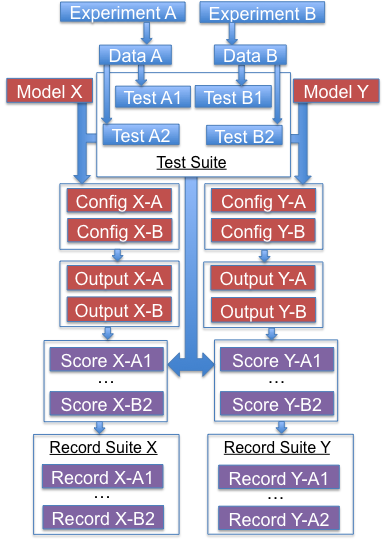
\includegraphics[scale=0.5]{sciunit_flowchart.png}
\caption{Workflow in \textit{SciUnit}. \scriptsize{i) Each experiment generates data, ii) From each set of data, many validation tests can be generated from test families (not shown); an ensemble of tests (from data within or across experiments) forms a test suite.  iii) Tests enumerate capabilities required for models to take them, and provide metadata used to configure models for execution.  iv) Model execution output is checked against test rules to produce a score.  Some test scores are not indicated here (…) for clarity.  v) The score establishes a validation record for that model+test combination.  An ensemble of records for one model is a record suite, and summarizes the scope and validity of the model.}}
\label{fig:sciunit_flowchart}
\end{wrapfigure}

A validation test in \textit{SciUnit} is an instance of a Python class implementing the \verbx{sciunit.Test} interface. Classes that implement this interface must contain a \verbx{run_test} method that receives a model as input and produces a \verbx{sciunit.Score} (a normalized score) as output. The capabilities that the model must possess in order for the test to operate correctly are given using the \verbx{required_capabilities} attribute. In many cases, several tests will have a similar form, differing only by a choice of parameters or by association with a particular dataset. Such parameterized \textit{test families} correspond to subclasses of \verbx{sciunit.Test}.  One \textit{test} is an instance of that subclass, with the needed parameters as constructor arguments. 

In Figure \ref{fig:rate_test}, the \verbx{RateTest} class implements a test family that compares the output "firing rate" (action potentials per second) of a neuronal model, driven by a given somatic input current, to an empirical mean and standard deviation (s.d.) of the firing rate derived from a set of replicated experiments. The test produces a boolean score indicating possible agreement within one s.d. of the empirical mean. The input currents, mean, and standard deviation are provided as constructor arguments on line 2 (constructors are named \verbx{__init__} in Python.) This parameterization creates a test from the \verbx{RateTest} test family.  On lines 6-9, the \verbx{required_capabilities} are listed: the model must be able to take a current as input and produce firing rates as output. These \textit{capabilities} are used in the \verbx{run_test} method, on lines 11 and 12 respectively, to execute the model against the provided current. The resulting firing rate is compared to the empirical mean and s.d on line 17 and a boolean score is produced on lines 18-22. In addition to the boolean value itself, the score also contains metadata that may be useful to scientists wishing to examine the result in detail. In this example, we save the model's output firing rate and the provided mean and s.d. alongside the result, by specifying the \verbx{related_data} parameter.
\todo{Check line numbers above.}  

\todo{What about non-binary tests?}

%Jonathan: 
%Regarding binary tests, the proposal does say "Validation is ultimately pass/fail, but in some cases the result generated in this phase also includes a continuous %statistic so that models can be ranked."  So non-binary results are part of the proposal, but they seem to be de-emphasized.  Of course pass-fail may be the best %way to capture results for some experiments; and sometimes even if the experimental result is continuous, a binary choice may be the most useful way to %analyze it.  But if a continuous result is sensible, wouldn't it make sense to put it on equal footing with a binary result in the framework?

%Josh:
%Why are the tests binary (i.e. they return a boolean value)? Isn't
%the stochastic nature of science better suite to a score? A model
%doesn't match or not match the data, it matches it with some
%precision. Why not return a floating point number between 0 and 1.

To create a validation test, a scientist instantiates the RateTest class with a particular mean, standard deviation and input current (I, not shown):\\
\vspace{-7px}\\\verbx{CA1_cell_rate_test = RateTest(mean=18.0, std=40.0, input_current=I)}\\\vspace{-7px}
\\
The test is then executed against a model instance (described below), using the \verbx{sciunit.run} function:\\
\vspace{-7px}\\\verbx{score = sciunit.run(CA1_cell_rate_test, CA1_cell_model)}\\\vspace{-7px}
\\
The \verbx{sciunit.run} function operates in three phases, implementing the abstractions from section \ref{sec:validation_tests}:
\begin{enumerate}
\item Capability Checking: The model is verified as capable of taking the test by checking each capability in the test's \verbx{required_capabilities} attribute.
\item Test Execution: The test's \verbx{run_test} method is called to execute the model and cache output.
\item Output Validation: \verbx{run_test} returns an instance of a \verbx{sciunit.Score} subclass containing a goodness-of-fit metric between the model output and the data used to instantiate the test.  Here the goodness-of-fit is all-or-none, i.e. pass/fail.  
\end{enumerate}
\hspace{-0px}Any errors that occur during this process are reported by raising an appropriate exception.

\subsection{Test Suites}
A test suite is a collection of tests designed to validate a model against several mutually coherent requirements:\\
\vspace{-7px}\\\verbx{spike_tests = sciunit.TestSuite([SpikeWidthTest, SpikeHeightTest])}\\\vspace{-7px}
\\
When a test suite is executed against a model, it produces summary data that can be shown on the console or visualized by other tools, such as the web application described in the next section. A test suite can also be used to compare multiple models (described below), producing a table as in Table \ref{table:record_matrix}.

\subsection{Candidates and Capabilities}
A \textit{candidate} is the entity to be tested.  In practice, this will usually implementat a particular scientific model, so \textit{candidate} and \textit{model} can be used interchangeably; we distinguish them to allow for the possibility that a candidate itself be a dataset subject to testing.  For clarity, we will refer to candidates as models herein.  A model is represented by an instance of a class inheriting from \verbx{sciunit.Candidate}.  In many cases, models can be grouped into parameterized \textit{model families}, as with tests, with parameters passed to an analogous subclass constructor.
\todo{What does it mean for "a candidate itself be a dataset subject to testing"?}

In order for a model to be tested, it must have certain \textit{capabilities} that the test requires.  That is, the model must be capable of taking certain kinds of input and generating certain kinds of output that the test will use to evaluate its validity.  A \textit{capability} is a contract guaranteeing that a model is able to produce results of a particular form. We model capabilities as Python classes containing unimplemented methods. In other object-oriented languages, this corresponds to an \textit{interface} or an abstract class.  

Let us consider the capabilities of a model publicly available on the Open Source Brain website \cite{osb_ca1_url}.  In the system being modeled, recorded data consists of the somatic membrane potential of a pyramidal neuron from area CA1 of the hippocampus, and the stimulus consists of somatically-injected current.  This somatic membrane potential includes action potentials, the rate of which is known in neurophysiology as the "firing rate".  Corresponding model capabilities might include \verbx{ReceivesCurrent}, \verbx{ProducesFiringRate}, and \verbx{TimeIntegrable}, the last of these indicating that the model can be integrated over time.    

Many capabilities must be enumerated to span a community's modeling formalisms. In the simple example we present here, these three capabilities suffice.  As two of them are domain-specific (to neuroscience), we place them not in \textit{SciUnit} itself but in \textit{NeuroUnit} in the module \verbx{neurounit.capabilities}.  In contrast, \verbx{sciunit.capabilities} contains only domain-independent model capabilities like\\ \verbx{TimeIntegrable}.

A model is represented by an instance of a class inheriting from \verbx{sciunit.Candidate}.  In Figure \ref{fig:ca1_model}, the CA1 cell model family implements the above capabilities, which both permits testing and importantly determines which tests are within its scope.  A models implemented at a different level of detail may have different capabilities and thus be eligible to take a different set of tests.  

\begin{figure}
\caption{A candidate class corresponding to a CA1 Pyramidal Cell model from Open Source Brain}
\label{fig:ca1_model}
\begin{python}
class CA1PyramidalCellModel(NeuroConstructModel,
				            capabilities.ReceivesCurrent):
	"""CA1 Pyramidal Cell model from /neuroConstruct/osb/hippocampus/
	CA1_pyramidal_neuron/CA1PyramidalCell"""
	def __init__(self,**kwargs):
		# Put any other initialization here.
		project_path = os.path.join(candidates.putils.OSB_MODELS,
									"hippocampus",
									"CA1_pyramidal_neuron",
									"CA1PyramidalCell",
									"neuroConstruct")
		candidates.NeuroConstructModel.__init__(self,project_path,**kwargs)
		super(CA1PyramidalCellModel,self).__init__(**kwargs)
\end{python}
\vspace{-18px}
\end{figure}

In Figure \ref{fig:ca1_model}, the model produces a firing rate after being provided a current.  The capabilities a model must implement are determined by its base classes; it multiply inherits some \verbx{sciunit.Candidate} subclass (here NeuroConstruct.Model, described in \ref{sec:neuroml_candidates}), and some number of \verbx{sciunit.Capability} subclasses.  The model then expresses methods (such as \verbx{set_current}) that override (and implement) the abstract, unimplemented methods provided in the corresponding \verbx{sciunit.Capability} subclasses.  Any capability the model inherits must have all if its associated methods implemented.  Failure to do so will result in a \verbx{NotImplementedError}, indicating a model scope less than claimed by its inheritance.  

A \textit{model family} is initialized with parameters (\verbx{i_leak} in the case of the model in Fig. \ref{fig:ca1_model}) to produce a \textit{model}.  A test does not specify these parameters, however a tester may nonetheless subject a range of models from a model family to the same test.  This is done by repeatedly instantiating the model with different parameters (for example, in a loop).  If a particular parameter value in the model is required for a test to be sensible, this can be expressed in the list of \verbx{required_capabilities}.  For example, if the test is only passable by models corresponding to a particular pharamacological milieu (e.g. with some fraction of ion channels of a certain type blocked), then \verbx{required_capabilities} might include \verbx{ModifiesConductance}, exposing a method \verbx{set_conductance}.  The test specification could also include run-time arguments for models, which could correspond to a waveform of injected somatic current, or alternatively to training data for models implementing completing algorithms.  Figure \ref{fig:sciunit_flowchart} illustrates the testing workflow, and Table \ref{table:glossary} provides definitions of terms.  
 
\begin{table}[h]\footnotesize
\caption{Glossary of Terms}
\label{table:glossary}
\begin{tabular}{| c | p{13cm} |}
\hline
Data & The measurements yielded by an experiment.\\ \hline  
Model & An executable function that aims to explain, reproduce, or predict experimental data.  More generally, a candidate.\\ \hline
Model Family & A class that generates a set of related model instances. Each model instance from one family differs according to the set of parameters (corresponding to a particular experimental design, or set of training data) with which it was initialized.\\ \hline  
Validation	 & The process of assessing the agreement between model output and experimental data.\\ \hline
(Validation) Test & A function that executes a model and scores the model’s output against a summary of experimental data. One experiment can inform the development of many tests.\\ \hline  
Test Family & A class that generates a set of related test instances.  Test instances from within one family differ only quantitatively, according to the data used to initialize them.  All tests from one family attempt to validate the same property of a model.\\ \hline
Test Suite & A collection of tests, each of which attempts to validate a different property of a model.\\ \hline  
Score & A value summarizing the performance of a model on a test. This can be a measure of the goodness of fit between model output and experimental data.\\ \hline
Scope & A list of tests that a model is eligible to take, indicating the range of experimental data that the model might be able to explain or replicate.\\ \hline
Capability & 	A contract that states that a model is able to produce results of a particular form. For example, a Hodgkin-Huxley neuron model is capable of producing a membrane potential time-series, whereas a model without a notion of voltage is not.\\ \hline
Record & An indication of the test score achieved by a model, along with any initialization conditions.\\ \hline
Record Suite & A list of records associated with a model.  This summarizes the scope and validity of the model.\\ \hline  
\end{tabular}
\end{table}

\subsection{\textit{SciDash} Development}
We have also begun work on the \textit{SciDash} web application, which point to models and tests and aggregate test results for scientific communities. A development version is currently live \cite{scidash_url}.  It is populated with models and tests from the educational illustration in Table \ref{table:record_matrix}.  This application has several key features.  \textbf{First}, it provides a "dashboard" view of the state of a field by displaying a matrix of records for selected model/test combinations, i.e. those stored in a given GitHub repository (Fig. \ref{fig:scidash_repo}.  \textbf{Second}, each record will link to the tests results (stored in the repository), displaying line-by-line the executed code and intermediate output statements, as well as the underlying models and tests.  One possibility is the use of the Sage notebook \cite{sagenb_url}, whose "worksheets" facilitate visualization and storage of executed code.  While Sage was written for Python, the notebook also supports the execution of code and visualization of outputs from other programming languages, making possible worksheets based on MATLAB, Mathematica, and other popular environments for modeling.  \textbf{Third}, a community-moderated comment section will allow test-makers and test-takers to discuss issues associated with each record.  Thus, disagreements about the appropriateness of a test can be openly aired and in many cases resolved.  We support open authentication via existing web applications (Google, Yahoo, Twitter, etc.), lowering the barrier to participation.  The \textit{SciDash} backend will consist of a MySQL relational database, updated regularly using the GitHub API to populate record matrices.  
\todo{More discussion of what SciDash will show about the test results}  

% Josh: In particular I'd like to
%see more discussion of the overview SciDash will give of the test
%results. Are all tests equal? What aggregation functions will you
%provide?How will a new user (or journalist as you suggest in one of
%the concluding sections) be able to reasonably quickly understand "how
%well" a model predicts the data?

% Section 4.
\section{Research and Development Plan}
In order to make immediate use of \textit{SciUnit} and populate \textit{SciDash} with models and tests, we will initially focus on \textit{NeuroUnit} development, to serve one discipline (neurophysiology) without compromising generalizability. This will enable rapid feedback from a familiar experimental community, guiding development.  

\subsection{Leverage of existing resources for the development of \textit{NeuroUnit}}
Here we describe standard neuroinformatics tools we have adopted to develop \textit{NeuroUnit} \cite{neurounit_url}.  

\subsubsection{Candidates from NeuroML Models}\label{sec:neuroml_candidates}
NeuroML is a standardized model description language for neuroscience \cite{gleeson_neuroml:_2010}. It permits many neurophysiological/neuroanatomical models to be described in a simulator-independent fashion, and executed across many popular simulators due to inter-conversion capabilities of the NeuroML API.  Because NeuroML is an XML specification, model descriptions can be validated for correctness and queried for model properties and components, exposing potential capabilities.  It is ideal for model sharing, curation, and for answering both \textit{what} and \textit{how} programatically.  

NeuroConstruct \cite{neuroconstruct_url,gleeson_neuroconstruct:_2007} is a simulation manager that takes NeuroML models and hands off simulation to supported neural simulators. To this end, \textit{NeuroUnit} offers a \verbx{sciunit.Candidate} subclass called \verbx{NeuroConstructModel}, instantiated with the path to a NeuroML model.  Because NeuroML can describe such a wide range of models, \verbx{NeuroConstructModel} makes few assumptions about them: that they each is \verbx{TimeIntegrable}, and \verbx{HasMembranePotential}.  It is subclassed to test \textit{specific} NeuroML models (Fig. \ref{fig:ca1_model}). 

The Open Source Brain project (OSB, \cite{osb_url}) curates many models described in NeuroML. OSB-curated projects are converted from their native format into NeuroML, and run on major neural simulators \cite{neuron_url,genesis_url,nest_url,moose_url}. Concordance between model output (beginning with the NeuroML description) and reference output (from native simulator source files) is reported for each model.  Thus, OSB is an excellent source of models that, in addition to being open source, are sufficiently described to enable validation.   The hippocampal CA1 pyramidal cell is commonly modeled, and we implement one such model hosted on OSB \cite{osb_ca1_url} by simply declaring a \verbx{CA1PyramidalCellModel} class , deriving from \verbx{NeuroConstructModel}.  This basic implementation simply "wraps" the functionality of the existing model, and only the code shown in Fig. \ref{fig:ca1_model} is required.  All OSB models, and indeed any NeuroML model, can be tested similarly.  Working together with OSB is part of our \textbf{first collaboration}, and our integration efforts can be publicly tracked \cite{neuroconstruct_rgerkin_url}.  

Spanning a range of scales and original development environments, all OSB models are formally described using NeuroML, as are all model components and sub-components, such as cells, ion channels, calcium stores, etc.  These models are regularly executed on OSB servers to ensure that their output remains consistent as they are updated.  Therefore, OSB can confirm that they \textit{do} work, while linked journal articles, on-site wiki, and code inspection can establish \textit{how} they work. However, there is no mechanism for establishing \textit{how well} they work, i.e. how well the models accord with data.  \textit{SciUnit} fills this gap by helping OSB (and the larger biology community) assess models using data-driven tests in the \textit{NeuroUnit} library.  \textit{SciUnit} can be applied similarly to other biology sub-disciplines using \textit{NeuroUnit} analogues written by the corresponding communities.    
\todo{Does this mean that SciDash-OSB would be a repository?}

\subsubsection{Capabilities from NeuroTools}
NeuroTools \cite{neuralensemble_url} is a Python library supporting tasks associated with analysis of neural data (or model output), such as membrane potential time series, spike trains, etc. It is an open source and actively developed project, containing reliable algoithms on which to base neurophysiology tests.

We use NeuroTools to implement \textit{SciUnit} capabilities in \textit{NeuroUnit} (Fig. \ref{fig:neurounit_example}).  For example, a NeuroTools \verbx{AnalogSignal} object (e.g. a membrane potential time series) has a threshold detection method that returns a NeuroTools \verbx{SpikeTrain} object.  A \textit{NeuroUnit} \verbx{HasSpikeTrain} Capability requires that  \verbx{getSpikeTrain} method be implemented.  \verbx{NeuroConstructModel} does so by placing \verbx{AnalogSignal.threshold_detection} inside \verbx{getSpikeTrain}.  Many such NeuroTools objects are similarly exchanged between \verbx{NeuroConstructModel} methods.  This simplifies test writing, since basic model output properties are obtained trivially using NeuroTools object methods, and these NeuroTools objects are easily extracted from model output using candidate models subclassing \verbx{NeuroConstructModel}.  

\subsubsection{Reference Data for Tests from NeuroElectro}
Answering \textit{how well} requires validation testing against data. The NeuroElectro project \cite{neuroelectro_url} is an effort to curate all published single cell neurophysiology data \cite{tripathy_neuroelectro:_2012}.  Currently, up to 27 electrophysiological properties are reported for 93 cell types, spanning $>$ 2000 single pieces of published data extracted from article tables.  \textit{NeuroUnit} tests are easily constructed using the NeuroElectro API for reference data. Tests can be based upon data from single journal articles, or from ensembles of articles with a common theme (e.g. about a particular neuron type).  The former is illustrated in Figure \ref{fig:neurounit_example}.  Associated statistics of that data (e.g mean, standard error, and sample size) are attached and enable judgement of model output according to a chosen scoring mechanism.\todo{Should there actually be an example of workflow with NeuroElectro here?} While NeuroElectro alone cannot judge all model aspects, it can serve to validate basic features of many models, such as resting membrane potential, action potential width, after-hyperpolarization amplitude, etc.  As NeuroElectro is the only publicly curated source of such data, it represents a key component for \textit{NeuroUnit} test constuction.  Continued development of the NeuroElectro API, through which data are systematically exposed to test authors, represents our \textbf{second collaboration} \cite{neuroelectro_dev_url}.  

\subsubsection{A Complete Pipeline}
Although the tools above do not exhaust the possible sources of models, capabilities, and test data, they provide an immediate point of entry into the neurophysiology community and powerful demonstration of our proposal.  In the \textit{NeuroUnit} repository \cite{neurounit_url} is a runnable script (\textit{examples.py}) demonstrating a complete testing pipeline.  It (1) selects an OSB model; (2) simulates it using NeuroConstruct; (3) tests the widths of the resulting action potentials, extracted and computed using NeuroTools, against NeuroElectro data downloaded on-the-fly, using a \textit{NeuroUnit} test class called \verbx{SpikeWidthTest}; and (4) computes and prints a test score.\todo{Show a code block for this.}

\subsubsection{Creating New Candidates, Capabilities and Tests}
\textit{NeuroUnit} provides base classes to enable rapid generation of candidates, capabilities, and tests for neurophysiology data.  However these objects can also be created from scratch, requiring only adherence to the core \textit{SciUnit} interface.  For example, a Candidate could implement an \verbx{integrate} capability method by wrapping execution of a MATLAB script and a \verbx{get_spikes} capability method by parsing a .csv file on disk; and a test could be initialized using empirical spike rates collected in the lab. 

\subsection{Public Dissemination}
Concurrent with these efforts, we are creating a community portal (\textit{SciDash}) written using Django, a Python web framework.  The source code for the web application and the framework will be developed openly and released under a permissive open source license continuously. An open release, rather than one implemented solely behind our portal, supports labs or groups that want to test models on their own machines as they are being developed, or to compare competing models on unreleased data.  So long as a GitHub repository has been forked from the main SciDash repository \cite{scidash_repo_url}, and is publicly visible (the default in GitHub), it will be automatically indexed by and visible on SciDash. The community portal will thus point to models and tests as they become available, and display corresponding test results.  Thus, there will exist a dedicated resource for evaluating the validity of models, and the progress of the SciUnit initiative, including the rate of community adoption, will be transparent.  

The SciDash portal will host scripts that read thes GitHub repositories, run any outstanding tests on new or existing models, and format the results.  In order to quickly populate SciDash with repositories that are both useful and illustrative, we will recapitulate the results of some "settled" competitions in SciDash format, i.e. we will encode the competition rules as tests and SciDash will then index the results.  There are several examples of such settled competitions which have publicly available rules, entries, and published results against which to check \cite{jolivet_quantitative_2008}.  
% The above in response to Josh's comment: 
% Josh: How are you validating SciDash? I don't see any discussion of how
%you will determine if it is successful. One suggestion: perform a
%qualitative use case analysis of the application.

\subsection{Project Milestones}
\begin{description}
\item[Year 1:] We will continue \textit{SciUnit} core development, and implement \textit{NeuroUnit} tests using NeuroElectro data and capabilities using NeuroTools functions.  At the end of this period we will have a manuscript in review, describing the idea and preliminary results, and have released a stable \textit{SciUnit} Python module for general use. 
\item[Year 2:] We will automating model testing for OSB, greatly increasing the number and scope of models tested.  We will continue to define \textit{SciUnit} model capabilities via collaborative development of NeuroTools, and aggregate new community-provided datasets to test the capabilities of OSB models.  At the end of this period, OSB will support automated testing and result summaries, and \textit{SciDash} will contain a broad array of models and tests to browse and visualize.  
\item[Year 3:] We will extensively documentation \textit{SciUnit} and associated tools to encourage adoption.  We will actively promote its use at conferences and workshops.  We will continue to write tests and specify (existing, published) models in NeuroML for execution and testing. At the end of this period we will have another manuscript in review, describing the results of the research program and promoting the \textit{SciDash} portal.  \textit{NeuroUnit} will contain a sufficient array of usable tests to motivate considerable community interest and serve as an example for developers in other biology disciplines.  
\end{description}
\subsection{Challenges}
Here we describe theoretical and practical challenges to implementation, and how they can be overcome.

\subsubsection{Participation from Modeling Communities}
Modelers may not want to expose model capabilities, a requirement of test-taking.  We anticipate four solutions: \textbf{First}, interfacing a model to \textit{SciUnit} requires only implementing selected model capabilities.  This means identifying model outputs that satisfy a capability, and returning their values.  It also means identifying model inputs used for parameterization, or run-time arguments, and providing a means to set them.  However, each of these procedures may require only one line of code.  Importantly, the modeler is not required to expose or rewrite any model flow control.  \textbf{Second}, we will support multiple environments automatically by using NeuroML \cite{gleeson_neuroml:_2010}, a simulator-independent model description language. As we have shown, models described in NeuroML will be easy to test using \textit{NeuroUnit}.  Efforts are also underway to automate generation of NeuroML descriptions from the source code used by models written for popular simulators (Gleeson, personal communication).  For the NEURON simulator, this process is largely complete.  Thus for a large and growing number of models, modeler effort is already close to zero.  \textbf{Third}, modelers have a strong incentive to use \textit{SciUnit} to demonstrate in an umambiguous and public way that their models are consistent with data.  Participation in public modeling competitions (see section \ref{sec:existing_efforts}) illustrates this incentive.  Fourth, modelers have a strong incentive to use \textit{SciUnit} during development (see TDD, above) to guarantee that on-going development does not break the correspondence between the model and the system it explains.  A suite of popular tests will represent a "gold standard" by which modelers can judge their progress during development.

\subsubsection{Participation from Experimental Communities}
Experimentalists may not want to write tests derived from their data, or are not comfortable with writing code.  We anticipate three solutions: \textbf{First}, rather than demand the use of special formats for data, each test will need only a list of required model capabilities (for selecting eligible models), essential experimental metadata (as run-time arguments to models) and a statistical summary of data (for scoring results) be written into each test.  By definition each unit test is focused, and does not require the ability to do arbitrary computations on a data set.  Suppose that one has evoked by intracellular current injection in a cell 100 action potentials and wishes to write a test concerning the width of these action potentials.  Writing the test then consists of selecting ReceivesCurrent and ProducesActionPotentialShape capabilities (one line of code each), typically computing the mean and variance of action potential widths in the data (one line of code), specifying the parameters of the current injection, e.g. the amplitude and the duration (two lines of code), and finally selecting a scoring mechanism from \verbx{sciunit.scores}, e.g. (colloquially) "Must be $<$ 1 standard deviation of the mean value" (one line of code).  Most of the heavy-lifting is done by the interface.  An example can be found in \verbx{neurounit.tests.SpikeWidthTest}.  \textbf{Second}, as data-sharing becomes more ubiquitous, this task can be distributed across a large number of scientists, including non-experimentalists interested in data analysis or testing their own models. \textbf{Third}, a large number of tests can be automatically generated using the NeuroElectro API, and the continued emergence of systematically organized data repositories will expand these possibilities. \textbf{Fourth}, a strong incentive to write tests for one's data exists: the ability to identify models that explain one's data, giving the data clear context and impact. 

\subsubsection{Diversity of Levels and Kinds of Models and Data}
How can one framework deal with so many topics in biology?  \textbf{First}, we solve this by providing an interface that allows modelers to express the capabilities which their model possesses.  The set of all capabilities so described determines the range of tests that can be executed, and the set implemented by one model determines the range of tests that the model can take.  Hierarchies of scale are embedded in the inheritance of capability classes.  For example, an answer to the question "Does this model have action potentials" requires a "yes" answer to the question "Does this model have neurons".  Consequently, the incompatibility of a test-requiring-action-potentials for a model-lacking-neurons is known without explicit tagging.  Conversely, a model with a \verbx{HodgkinHuxley} capability also inherits a \verbx{VoltageGated} capability, because the former implies the latter. \textbf{Second}, expressing models in NeuroML naturally addresses diversity of levels (i.e. scales) because NeuroML is developed in "levels", with a hierarchical organization.  Thus, models can be sub- or supersets of other models.  Analogous hierarchies exist in SED-ML \cite{sedml_url,hucka_systems_2003}, a general systems biology markup language. \textbf{Third}, testing across levels could also be implemented using the "Representional Similarity Analysis" (RSA) framework \cite{kriegeskorte_representational_2008}, requiring only that a model be capable of responding to a defined set of inputs (e.g. stimuli).  A "similarity matrix" for responses within a model and across inputs defines a unique signature for that model, and can be the intermediate output of a test.  Model scale becomes irrelevant, because test scores are based on goodness-of-fit between similarity matrices for model and experiment -- these matrices can be compared directly no matter the model scale because their size depends only on the number of test inputs, not on system detail.  

\subsubsection{Appropriateness of Models for Validation}
Not all models attempt to reproduce experimental findings.  Some models serve as proof of concept that a dynamical system with have certain properties.  We do not intend to challenge these proofs; however, tests that abstract away most experimental details can inform and illuminate such models.  For example, rather than encoding specific experimental stimulus and response values, a test could simply evaluate a mapping between sets of numbers.  Some abstract models may have unexpected homology to that mapping, thus highlighting the relevance of such models where it may otherwise have been missed.  Alternatively, a model may make specific experimental predictions, but require significant contextual information not provided by a test.  Rather than fail such models, we give them an "incomplete", i.e. no record of the test result is generated for such a model, in accordance with the model's scope.  

\subsubsection{Arbitrary Scoring Criteria for Tests}
A raw test score is computed from goodness-of-fit to data, and a pass/fail mark from that score.  At both stages there is room for arbitrary design choices that will benefit some models at the expense of others.  \textbf{First}, many goodness-of-fit functions have, for a given input set, identically rank-ordered outputs, meaning that such design choices will rarely cause an otherwise passing model to fail and vice versa.  For example, the function mapping Z-scores to p-values in monotonic.  Indeed, one may ignore quantitative differences between model scores, with focus given instead to the rank ordering of those scores. \textbf{Second}, since test repositories are open (e.g. Fig. \ref{fig:scidash_repo}), it is straightforward to clone a test and change the statistical choices used for scoring.  With each test transparent, a community can decide which test version is most appropriate.  This process will be open and documented on \textit{SciDash} via GitHub.  Thus, the community decides on what models should do, and the framework then determine whether it does those things. 

\subsubsection{Reliability of Data Underlying Tests}
Unreliable data will lead to tests that even perfect models will not pass. \textbf{First}, it is incumbent upon the community to evaluate experimental design and techniques involved in producing data, and to discount data produced using questionable methods.  \textit{SciDash} will support community moderation, permitting users to rate and comment on tests, indicating their concerns.  Data may reflect artifacts of experimental preparation, such as electrode type or recording temperature, but this metadata is increasingly visible e.g. on NeuroElectro, so test writers may identify those data appropriate to the system being modeled, and this metadata can be attached to resulting test scores.  \textbf{Second}, models cannot fit perfectly to data when that data is a random draw of finite sample size from a "true" distribution.  This can be addressed by making uncertainty in the data explicit, or by asking how well a data set can validate its own experimental replications \cite{kriegeskorte_representational_2008}.  Since a model cannot validate better (in expectation) than an identical experiment, test scores may be modified to reflect that goodness-of-fit matching that of experimental replication represents a "perfect" score.  
\todo{How will the "rating" of a test be reflected into a SciDash view of a model?}

\subsubsection{Computational Efficiency}
Large models may execute slowly, and subjecting such models to many tests could be computationally intensive.  To lighten the burden, we prioritize minimal re-execution of the same model in \textit{SciUnit}'s design.  Sets of tests requiring as input the same model output only require the model to be executed once.  Model output, generated by execution of the first test, can be cached for use by similar tests.  For example, model execution instances could be stored as Sage worksheets in the corresponding repositories.  We have also implemented caching in the \verbx{sciunit.utils} module, by storing candidate instances and associated execution data in an optional database backend.  

\subsubsection{Occam's Razor}
A model's ability to explain data is typically weighed against its complexity -- simpler models being better, \textit{ceteris paribus}.  Model complexity has many definitions, so \textit{SciUnit} will report several complexity metrics, including: 1) the number of lines, instructions, or operations in the model; 2) memory use during model execution; 3) average CPU load during model execution; 4) number of model parameters.  Larger, longer, and more expressive models may be considered more \textit{complex} (\cite{mccabe_complexity_1976}).  The tradeoff between model validity and complexity can be reported in tabular form (e.g. Table \ref{table:record_matrix}); alternatively, a scatter plot, with the "best" models being in the high validity / low complexity corner of the plot, may be informative.  The set of models which \textit{dominate} all others, i.e. that have higher validity and lower complexity than their rivals, can be represented as a "validity vs. complexity" front, showing those models with the highest validity for a given level of complexity, a visualization familiar from the symbolic regression package Eureqa \cite{schmidt_distilling_2009}.  One then weighs the relative importance of validity vs. complexity for one's application.  

\subsubsection{Expansion Into Other Areas of Biology}
After proving its utility in neurophysiology, we would like \textit{SciUnit} to expand across neuroscience and then into other biological sciences.  Since the core framework is discipline-agnostic, the only obstacles are community participation and model description.  As with neurophysiology, community participation begins with enumerating the capabilities relevant to a sub-discipline, and then writing tests.  Model description can expand within NeuroML (which already covers multiple levels and approaches within neuroscience) and \textit{NeuroUnit} tools can begin to incorporate libraries for neuroimaging (NiBabel \cite{nibabel_url}), neuroanatomy (NeuroHDF, \cite{neurohdf_url}) and other sub-disciplines.  SED-ML \cite{hucka_systems_2003,sedml_url} will facilitate expansion outside of neuroscience.  This transition will be facilitated by parallel efforts in the NeuroML community to interface with SED-ML (Crook, unpublished).    

% Section 5.
\section{Broader Impacts}
\subsection{Education}
The cornerstone of basic science education is learning the scientific method.  However, the process by which the scientific method is applied in practice may be too informal to be recognizable to students.  \textit{SciDash} will provide a visible example of the scientific method in practice, determining which hypotheses (models) can withstand the scrutiny of evidence (can pass tests).  Revision of hypotheses to match evidence will also be transparent, as \textit{SciDash} will show and optionally group test results for model variants.  Github tracks and exposes revisions, which would include revisions to models as they are refined to match experiments.  The ability to visualize the scientific method at work from any computer in the world will represent a major step forward in science education.  

As a pedagogical tool, we will provide SciDash repositories for historical case studies.  We show an example in Table \ref{table:record_matrix}: consider 5 astronomical models and 4 validation tests derived from relevant data.  This record matrix, showing implied test scores, recapitulates the history of cosmology, showing the scientific method to be an on-going process.  The Geocentric model of Claudius Ptolemy (\cite{ptolemy_almagest_150}) passes a test derived from Babylonian records of planetary motion.  Ptolemy's model fails all other tests shown here, including one constructed from Tycho Brahe's more meticulous measurements of planetary motion (\cite{kepler_rudolphine_1627}), being inconsistent with Ptolemy's notion of perfectly circular orbits.  The Copernican Heliocentric model (\cite{copernicus_revolutionibus_1543}) also predicts circular orbits and thus fails Brahe's test, but is far simpler than the Ptolemaic model, dispensing with notions such as "epicycles".  Kepler's laws of planetary motion permit and explain these elliptic orbits (\cite{kepler_astronomia_1609}), as well as Galileo's unanticipated discovery of moons taking elliptic orbits around Jupiter (\cite{galilei_siderius_1610}).  Newton's gravitational model passes these tests and does so by more succinctly by unifying Kepler's laws under one principle: gravity (\cite{newton_philosophiae_1687}).  Newton's model was challenged by the observation of perihelion precession of Mercury (\cite{le_verrier_lettre_1859}).  General Relativity resolved this problem (\cite{einstein_foundation_1916}).  Interestingly, Einstein explicitly proposed 3 tests of his theory, of based on Le Verrier's precession data.  While this account may be simplistic compared with testing practice in modern biology, it would be appropriate for teaching the scientific method to a high school or college student.  SciDash will index and highlight case studies such as these for teaching.  

These examples will also serve as a general introduction to SciUnit specifically, which will help with our second outreach effort: engaging students in model building and validation through focused competitions built on SciUnit and tracked using SciDash.  Dr. Aldrich regularly teaches a computer programming class in which students are asked to create artificial lifeforms that must achieve specific objectives.  He will update the curriculum to... \todo{Cyrus, could you elaborate}.  Dr. Crook teaches a computational neuroscience class in which students build models of spiking neurons.  She will being using NeuroUnit to validate that the models achieve the desired output.  In both cases, the use of the SciUnit framework during (and not simply after) development, i.e. test-driven development, will be encouraged.  We believe that adoption of this framework will be most rapid when students learn to test their models as a habit and not an after-thought.  To this end, Dr. Gerkin will sponsor a Google "Summer of Code" application \cite{summerofcode} to fund interested high school students to improve upon existing models in areas of student interest using SciUnit.  The sponsor ultimately selects from among the applicants, and we will actively seek minority and female applicants for this project.  

\begin{wraptable}[10]{r}{0.7\columnwidth}
\caption{A record matrix illustrating models and data-driven tests from the history of cosmology. Each row is a model; each column is a test.}
\label{table:record_matrix}
\begin{tabular}{| c | c | c | c | c | c | c }
\hline
		& \textit{Complexity} & \textbf{Babylon} & \textbf{Brahe} & \textbf{Galileo} & \textbf{Le Verrier} \\ \hline
	\textbf{Ptolemy} & Medium & \textcolor{ForestGreen}{Pass} & \textcolor{Red}{Fail} & \textcolor{Red}{Fail} & \textcolor{Red}{Fail} \\ \hline
	\textbf{Copernicus} & Low & \textcolor{ForestGreen}{Pass} & \textcolor{Red}{Fail} & \textcolor{Red}{Fail} & \textcolor{Red}{Fail} \\ \hline
	\textbf{Kepler} & Medium & \textcolor{ForestGreen}{Pass} & \textcolor{ForestGreen}{Pass} & \textcolor{ForestGreen}{Pass} & \textcolor{Red}{Fail} \\ \hline
	\textbf{Newton} & Low & \textcolor{ForestGreen}{Pass} & \textcolor{ForestGreen}{Pass} & \textcolor{ForestGreen}{Pass} & \textcolor{Red}{Fail} \\ \hline
	\textbf{Einstein} & High & \textcolor{ForestGreen}{Pass} & \textcolor{ForestGreen}{Pass} & \textcolor{ForestGreen}{Pass} & \textcolor{ForestGreen}{Pass} \\ \hline
\end{tabular}
\end{wraptable}
\leavevmode

\subsection{Journalistic Media}
When reporting on new scientific theories, lay members of the media have no reliable way to determine the importance or quality of such theories.  Direct consultation of scientists may be unreliable, due to bias or lack of focused expertise.  However, \textit{SciDash} would -- for any model that it covers -- provide an unbiased way for media members to identify the scope and validity of a model, and contrast this with previous efforts.  With the original sources of models and tests well-documented, contributors could be contacted for comment or explanation.  Site-embedded commentary provided by modelers and test-writers should also be a helpful media resource.  

The competitive nature of \textit{SciDash} will be appealing both to scientists and to the lay community.  Competitions for machine learning, solar cars, and autonomous vehicles already draw considerable media coverage and we believe that the brain is of no less interest to the public.  Public competitions also welcome teams who may not yet have academic credentials, such as students, both to learn the craft and possibly to demonstrate key insights not previously recognized in the professional scientific community.  

Because the project is open at every level, links embedded in social media will provide a path of minimal resistance for anyone to explore the project and the models and tests that give it life.  In the third year we plan to actively promote the idea by getting coverage in media of interest to the targeted communities, via Twitter and popular blogs that increasingly cover "open" developments in science.  While such avenues may not have much import to senior scientists, they are critical to communicating with the next generation of scientists who have not yet established a go-to modeling workflow.   

% Here is a section from one of Sharon's grants that we could borrow from:  

%Educational outreach: The PI, graduate students, and undergraduate students funded through
%this proposal will work with high school science and mathematics teachers from a local high 
%school to develop structured activities that are aligned to the Arizona Education Standards, 
%with the goals of developing innovative, inquiry-based science education and serving minority 
%students. The activities will be modular in nature and will emphasize inquiry-based instruction 
%related to major concepts relevant to the proposed research. Some possible topics for modules 
%are  Insect Behavior and Learning,  Central Pattern Generators and Locomotion, and  Sensory 
%Adaptation. Each module will involve a set of coupled classroom active-learning sessions and 
%web-based computer simulation labs, focusing on the fundamentals of scientific reasoning, 
%mathematical skills, data analysis and relevant social impact within the context of the PI’s 
%research on neural adaptation. All personnel will contribute to the initial design of each module, 
%and the undergraduate students will perform the web development. Websites will be maintained 
%on the PI’s existing dedicated web server. One new module will be developed in each of years 1-
%3 of the grant.

%These activities will interface with an ongoing program (Borrow a Biologist) that has been 
%established to foster connections between under-represented students in the community, their 
%teachers, and faculty from Arizona State University's School of Life Sciences. With the aid of the 
%“Borrow a Biologist” program, a team of 2-3 biology and mathematics teachers will be recruited 
%each year. Teachers will participate in 1-2 day summer teacher 
%training sessions, and the PI and graduate student will visit the 
%classroom and provide on-going email contact with teachers and high 
%school students during the activities. Assessments of student 
%comprehension of relevant concepts, as well as of general attitudes 
%towards science and mathematics, will be made before and after the 
%planned activities using standardized questionnaires. Assessments 
%and teacher feedback will be used to adjust and improve the 
%classroom activities each year during the summer training sessions.  
%Classroom implementation of the modules will begin in year 2 of the 
%grant and continue through year 5. 
%After the modules have been refined, they will be incorporated into annual teacher training 
%workshops held at the Arizona Science Center starting in year 4 or 5 of the proposal. The 
%activities also will tie to a proven ASU webpage resource,  Ask a Biologist (http://
%askabiologist.asu.edu), which creates a vehicle for science literacy globally. The planned 
%activities will provide a unique opportunity to build ties with an educational institution and to help 
%assure its success, aiding in the scientific and mathematical development of under-represented 
%students. They will also serve as a source of hands-on training in science education and 
%mentoring for the graduate and undergraduate students involved in this project.
%Impacts on diversity in science and mathematics: The PI for this proposal works in an area 
%where women are under-represented and has demonstrated a commitment to mentoring other 
%under-represented groups in this field. She has served as a research advisor to eight 
%undergraduate and 11 graduate students, and of those 19 students, 13 are female, two are 
%Latina, and one is a Native American. Dr. Crook has also trained one postdoctoral researcher 
%who is Hispanic. Dr. Crook is involved with undergraduate curriculum development and training 
%for the NIH-funded MARC (Minority Access to Research Careers) Program in the School of Life 
%Sciences. She also mentors students from underrepresented groups at the graduate level, 
%participating in the activities of the Society for Graduate Women in Mathematics and the 
%Mathematical and Theoretical Biology Institute (MTBI). Under the direction of Dr. Carlos 
%Castillo-Chavez, the recruitment of graduate students through the MTBI %has raised the 
%percentage of underrepresented minority graduate students in mathematics at ASU from 
%2% to 20% over the last few years. Dr. Crook also has attended the Society for the Advancement 
%of Chicanos and Native Americans in Science Annual Meeting as a mentor and speaker.

% Jonathan said:
%"I think this is a good thing for us to do.  We could%
%* Sponsor workshops on evaluating scientific models in general, raising awareness of the need and building a community that might use our tools.
%* Give tutorials on our tools at scientific conferences
%* Organize competitions similar to those already mentioned in the proposal."

% Maybe we can co-opt and exiting computational neuroscience workshop and get a few hours/days of time there to teach SciUnit?  
% What about something like Woods Hole?  
% I think INCF might have money for these sorts of things.  

% Section 6.
\section{Personnel and Coordination}
\renewcommand{\theenumi}{\alph{enumi}}
A scientific software framework succeeds in proportion to its rate of adoption, which is driven in part by: \textbf{Relevance} to the needs of both experimental and theoretical scientists;
\textbf{Quality} of architecture and usability; \textbf{Conformance} to accepted data and modeling standards in the targeted communities; \textbf{Integration} with existing software tools; \textbf{Applicability} to outstanding questions in a field; \textbf{Community} access (i.e. an open and accessible internet presence). We have the appropriate team members to meet these criteria. 
\todo{Make sure to get each of these terms in the personnel descriptions below as often as possible without being annoying.}

\subsection{PIs}

\textbf{Richard C Gerkin, PhD} (25 hrs/week) has expertise in experimental and computational neurophysiology, neuroinformatics, and web development.  He will coordinate all project activities and be responsible for all output including code, databases, and manuscripts. He will also: coordinate with the NeuroElectro project and solicit other sources to obtain physiology data, format and annotate this data, and construct tests from the data (experience as both an experimentalist and a modeler will facilitate this objective (\textbf{Relevance})); write NeuroML-related bindings (e.g. \verbx{NeuroConstructModel}) (\textbf{Conformance}); subject models from OSB (and similar models publicly available) to these tests; develop and maintain the \textit{SciDash} website (\textbf{Community}); coordinate with the developers of OSB to implement automated \textit{SciUnit} testing.

\textbf{Sharon M Crook, PhD} (2 hrs/week) has expertise in mathematics, computational modeling, and neuroinformatics.  She will help interface \textit{NeuroUnit} to NeuroML and Open Source Brain. Access to the broader neuroscience community requires the use of an accepted model description standard.  We chose NeuroML due to its advanced state and broad coverage of multiple scales.  Dr. Crook is funded by NIH to maintain and support NeuroML and will help us use NeuroML for model specification (\textbf{Conformance}).  She will also assist with graduate training as needed.  

\textbf{Jonathan Aldrich, PhD} (2 hrs/week) has expertise in software engineering, software verification and validation, and human factors in software design. He will guide overall software architecture and supervise and train Mr. Omar.  His expertise in software design for science and engineering applications will be key in this role, and assure \textbf{quality}.  While Mr. Omar will be writing code, Dr. Aldrich will be providing guidance on the overall structure of the implementation.  Dr. Aldrich is already Mr. Omar's graduate supervisor (funded by other sources), but for this project Dr. Aldrich will take on the additional training responsibilities specific to the focus of this proposal.  

\subsection{Key Personnel and Collaborators}
\textbf{Cyrus Omar} (25 hrs/week) is senior graduate student with expertise in computational modeling in neuroscience, computer science, and software infrastructure for science.  He will guide core framework design and development and overall software architecture (\textbf{Quality}) and develop and maintain the core \textit{SciUnit} Python module.  He will get feedback from Dr. Gerkin about practicalities of model testing, which will inform revisions to the code.  

\textbf{R. Angus Silver, PhD} is a full professor with expertise in neurophysiology, computational neuroscience and neuroinformatics.  
A frequent collaborator of Crook, Silver maintains Open Source Brain (OSB), the largest standards-driven respository for models in neuroscience, for which he is funded by The Wellcome Trust.  
The OSB team has welcomed us to integrate \textit{SciUnit} into OSB for automated model testing (\textbf{Integration}).  
This exposes a wide range of neuroscience models specified in NeuroML (\textbf{Applicability}), and in turn exposes the project to the international neuroscience modeling community, serving as proof of concept for expansion into other areas of biology.  

\textbf{Shreejoy Tripathy, PhD} is a recent doctoral awardee with expertise in neuroinformatics, computational neuroscience, and data mining.  A frequent collaborator of Gerkin, Tripathy maintains The NeuroElectro Project, the largest data repository concerning electrophysiological properties of neurons.  He will help further integrate \textit{NeuroUnit} with NeuroElectro through API development, providing a wide range of data for testing neuroscience models.  

% Other potential collaborators (not necessarily all listed):
% Michael Hines (NEURON)
% OpenWorm guys
% Anyone with a modeling course
% Tim Verstynen
% Others?  

\subsection{Means of Coordination}
Dr. Gerkin trained in Pittsburgh and maintains ongoing collaborations with Dr. Aldrich, Mr. Omar, and Dr. Tripathy.  Dr. Gerkin works at ASU and regularly meets with Dr. Crook for "Math Biology" group meetings there.  Because the existing projects that form the basis for each collaboration are a) well-documented, and b) available under an open license, there should be no barriers to code sharing and collaborative development.  The popular and powerful Github platform will be used for code development and communication between developers.

% Section 7.
\section{Current and Previous NSF Funding}
\bfhead{Sharon Crook: [Intellectual Merit]} Sharon Crook was PI on NSF II-0613404, \$457,654, CRCNS: Behaviorally Relevant Neuronal Modification during Postembryonic Development, which was funded from 10/06 through 9/10. 
This work examined how dendritic structure and synapse distributions follow functional architecture principles that relate directly to a neuron's individual behavioral requirements in holometabolous insects, such as \textit{Manduca sexta} and \textit{Drosophila melanogaster.} 
The modeling and experimental activities focused on flight motoneurons, which generally transform from tonically firing larval crawling motoneurons into phasically firing adult flight motoneurons. 
This ongoing work has contributed to five publications so far \cite{hohensee, meseke, herrera-valdez_2012, ryglewski_2012, herrera-valdez_jcns_2013} with two more manuscripts in review, 
as well as seven published abstracts \cite{jennings_2007, herrera-valdez_2009, berger_2009, herrera-valdez_2010, smith_2011, berger_2012, berger_2013}. 
It also contributed to 12 poster or oral presentations at conferences and workshops. 
\bfhead{[Broader Impacts]} This grant also provided partial funding for training opportunities for four graduate students, including three women, and a postdoctoral researcher who is a Hispanic male. 
\\\\
\bfhead{Jonathan Aldrich: [Intellectual Merit]} In his work on NSF CAREER grant
CCF-0546550, ``Lightweight Modeling and Enforcement of
Architectural Behavior'' (2006-2010, \$500,000), Aldrich and his
students developed a new approach to extracting
run-time architectures from code and analyzing their
behavior, producing 12 major conference\footnote{note that in the field of computer science, major conferences are more prestigious than journals} and journal publications and numerous workshop papers,
including~\cite{AAC07,bierhoff07:modular_typestate_checking,AAN+08,AA07a,AA07b,AA08d,AA09a,AA09b,AB10}.
%More recently, Aldrich's work has been supported by NSF grants CCF-0811592 and CCF-1116907, 
%which have led to 8 major publications so far focused on language design and analysis approaches to verifying protocols of interaction between objects and proving safety
%properties of concurrent systems~\cite{beckman08:verifying_atomic,bierhoff09:plural,JA09,aldrich11:plaid,sunshine11:plaid,naden12:borrowing,hannesPlural,PradelAPI13}.  
%The DUE-1140760 project, just a year old now, has produced preliminary results on design education \cite{Cai13}.
\textbf{[Broader Impacts]} The NSF grant mentioned above, and 3 others, have contributed to the education of 11 Ph.D. students, including 4 women, and at least that many undergraduate or master's students.  The grants have also supported the development and release of a number of open-source tools,
including ArchJava \cite{ArchJava}, Plural \cite{pluraltool}, Crystal \cite{Crystal}, and SASyLF
\cite{SASyLF}. All of these tools, in addition to educational methodologies developed in the grants, have been used in education at
Carnegie Mellon and at other institutions.  Recognition of the broader impacts of
Aldrich's work on software architecture include the 2007 Dahl-Nygaard
Junior Prize and an ICSE most influential paper award.
%\todo{Document officially ends here for page count purposes.  Must be under 15 pages.}
\bibliographystyle{unsrt}
\nobibliography{references,references_crook,urls,references_ja}%\todo{Remove bibliography with nobibliography tag before submission}
%\listoftodos
\end{document}

